%% LyX 1.3 created this file.  For more info, see http://www.lyx.org/.
%% Do not edit unless you really know what you are doing.
\documentclass[english, 12pt]{article}
\usepackage{times}
%\usepackage{algorithm2e}
\usepackage{url}
\usepackage{bbm}
\usepackage[T1]{fontenc}
\usepackage[latin1]{inputenc}
\usepackage{geometry}
\geometry{verbose,letterpaper,tmargin=2cm,bmargin=2cm,lmargin=1.5cm,rmargin=1.5cm}
\usepackage{rotating}
\usepackage{color}
\usepackage{graphicx}
\usepackage{amsmath, amsthm, amssymb}
\usepackage{setspace}
\usepackage{lineno}
\usepackage{hyperref}
\usepackage{bbm}
\usepackage{makecell}
\usepackage{placeins}
\usepackage{subcaption}

%\renewcommand{\arraystretch}{1.8}

%\linenumbers
%\doublespacing
\onehalfspacing
%\usepackage[authoryear]{natbib}
\usepackage{natbib} \bibpunct{(}{)}{;}{author-year}{}{,}

%Pour les rajouts
\usepackage{color}
\definecolor{trustcolor}{rgb}{0,0,1}

\usepackage{dsfont}
\usepackage[warn]{textcomp}
\usepackage{adjustbox}
\usepackage{multirow}
\usepackage{graphicx}
\graphicspath{{../figures/}}
\DeclareMathOperator*{\argmin}{\arg\!\min}

\let\tabbeg\tabular
\let\tabend\endtabular
\renewenvironment{tabular}{\begin{adjustbox}{max width=0.95\textwidth}\tabbeg}{\tabend\end{adjustbox}}

\makeatletter

%%%%%%%%%%%%%%%%%%%%%%%%%%%%%% LyX specific LaTeX commands.
%% Bold symbol macro for standard LaTeX users
%\newcommand{\boldsymbol}[1]{\mbox{\boldmath $#1$}}

%% Because html converters don't know tabularnewline
\providecommand{\tabularnewline}{\\}
\renewcommand*{\arraystretch}{1.2}

\usepackage{babel}
\makeatother


\begin{document}

\renewcommand{\thefigure}{S\arabic{figure}}
\setcounter{figure}{0}
\renewcommand{\thetable}{S\arabic{table}}
\setcounter{table}{0}
\renewcommand{\theequation}{S\arabic{equation}}
\setcounter{equation}{0}

\section*{Supplementary Tables and Figures}

%%%%%%%%%%%%%%%%%%%%%%%%%%%%%%%%%%%%%%%%%%%%%%%%%%%%%%%%%%%%%%%%%%%%%%%%%%%%%%%%

\begin{figure}[h]
	\centering
	\includegraphics[width=0.9\textwidth]{lasso-ancestry-geno}
	\caption{}
	\label{fig:lasso-ancestry-geno}
\end{figure}

\begin{figure}[htbp]
	\centerline{\includegraphics[width=0.9\textwidth]{ratio-dist}}
	\caption{Relative predictive performance with UK compared to the PC distance with UK between centers of ancestry groups \cite[]{prive2020ancestry}. Relative performance values are the ones reported in Figure 1 of the main text.}
	\label{fig:ratio-dist}
\end{figure}

%%%%%%%%%%%%%%%%%%%%%%%%%%%%%%%%%%%%%%%%%%%%%%%%%%%%%%%%%%%%%%%%%%%%%%%%%%%%%%%%


\begin{figure}[htbp]
	\centerline{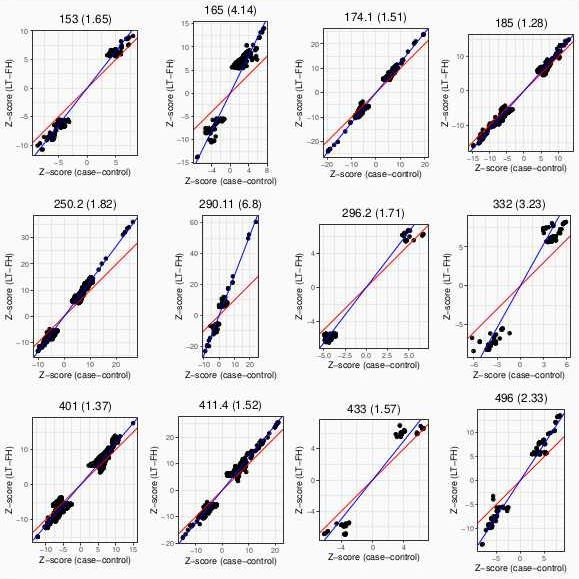
\includegraphics[width=0.95\textwidth]{power_LTFH}}
	\caption{Z-Scores from GWAS using case-control phenotypes and LT-FH phenotypes. Only variants with at least one Z-Score larger than 6 (in absolute value) are represented. The slope (in blue) is computed using Deming regression using the inverse of the absolute value as standard deviations.
	In the title are reported the phecode as well as this slope (squared), which we report as the power multiplier.}
	\label{fig:power-ltfh}
\end{figure}

\begin{figure}[htbp]
	\centerline{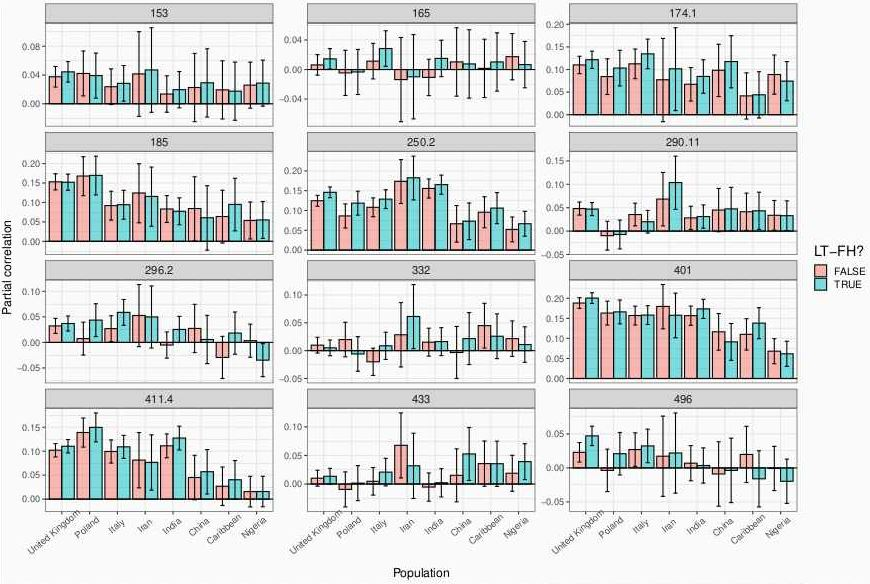
\includegraphics[width=0.9\textwidth]{lasso_LTFH}}
	\caption{}
	\label{fig:lasso-ltfh}
\end{figure}

\begin{figure}[htbp]
	\centerline{\includegraphics[width=0.9\textwidth]{lasso_LTFH2}}
	\caption{}
	\label{fig:lasso-ltfh2}
\end{figure}

%%%%%%%%%%%%%%%%%%%%%%%%%%%%%%%%%%%%%%%%%%%%%%%%%%%%%%%%%%%%%%%%%%%%%%%%%%%%%%%%

\begin{figure}[htbp]
	\centerline{\includegraphics[width=0.9\textwidth]{qc-plot-new-formula}}
	\caption{Comparison of the standard deviations (SD) computed from both genotypes and summary statistics for the 1000 most associated variants with bilirubin concentration. A) uses the previous formula $\text{sd}(\boldsymbol{G_j}) \approx \frac{\text{sd}(\boldsymbol{y})}{\sqrt{n ~ \text{se}(\hat{\gamma}_j)^2}}$ proposed in \cite{prive2020ldpred2} while B) uses the updated formula $\text{sd}(\boldsymbol{G_j}) \approx \frac{\text{sd}(\boldsymbol{y})}{\sqrt{n ~ \text{se}(\hat{\gamma}_j)^2 + \hat{\gamma}_j^2}}$ proposed here, which does one less approximation.}
	\label{fig:new-formula}
\end{figure}

%%%%%%%%%%%%%%%%%%%%%%%%%%%%%%%%%%%%%%%%%%%%%%%%%%%%%%%%%%%%%%%%%%%%%%%%%%%%%%%%

\clearpage


%%%%%%%%%%%%%%%%%%%%%%%%%%%%%%%%%%%%%%%%%%%%%%%%%%%%%%%%%%%%%%%%%%%%%%%%%%%%%%%%

\clearpage

\bibliographystyle{natbib}
\bibliography{refs}

\end{document}
